%
% Cover page
%

\title[Neutrino Physics]
{
  \Huge{Neutrino Physics}
}

\author[C.Andreopoulos] {
  Professor Costas Andreopoulos\inst{1,2}
}
\institute[Liverpool/STFC-RAL] {
   \inst{1} University of Liverpool,
   \inst{2} STFC Rutherford Appleton Laboratory\\
   \vspace{0.5cm}
   {\it {\color{magenta} A post-graduate student lecture course}}\\
   \vspace{0.2cm}
}
\date{\today}

\titlegraphic{
  
\includegraphics[height=25px]{./images/logo/liverpool.png}
  \hspace{3px}
  
\includegraphics[height=30px]{./images/logo/ral.png}
}

	



\begin{frame}[plain]
  \titlepage
\end{frame}


\begin{frame}{Structure of this course}

{\scriptsize

{\bf Prelude} \\

Part 1: {\bf Neutrino Oscillations} \\
\begin{itemize}
{\scriptsize
  \item {\color{magenta} Lecture 1: } Neutrino Oscillation Phenomenology
  \item {\color{magenta} Lecture 2: } Development of the 3 active $\nu$ scheme - Oscillations at the `solar' ${\Delta}m^{2}$
  \item {\color{magenta} Lecture 3: } Development of the 3 active $\nu$ scheme - Oscillations at the `atmospheric' ${\Delta}m^{2}$
  \item {\color{magenta} Lecture 4: } 3 active $\nu$ oscillations: Status, questions \& prospects
  \item {\color{magenta} Lecture 5: } Tensions in the 3 active $\nu$ scheme
}
\end{itemize}

Part 2: {\bf Neutrino Interactions} \\
\begin{itemize}
{\scriptsize
  \item {\color{magenta} Lecture 6: } Basics of electro-weak interactions
  \item {\color{magenta} Lecture 7: } Quasi-elastic neutrino scattering
  \item {\color{magenta} Lecture 8: } Resonance neutrino-production
  \item {\color{magenta} Lecture 9: } Deep inelastic scattering and neutrino-induced hadronization
  \item {\color{magenta} Lecture 10:} Coherent production of mesons
}
\end{itemize}

Part 3: {\bf Other topics} \\
\begin{itemize}
{\scriptsize
  \item {\color{magenta} Lecture 11:} Theory of neutrino mass and direct mass measurements
  \item {\color{magenta} Lecture 12:} Neutrino astrophysics
}
\end{itemize}

}
\end{frame}

%
%
%

\begin{frame}{Neutrinos in the Standard Model (SM)}

  \begin{columns}
    \begin{column}{0.30\textwidth}
      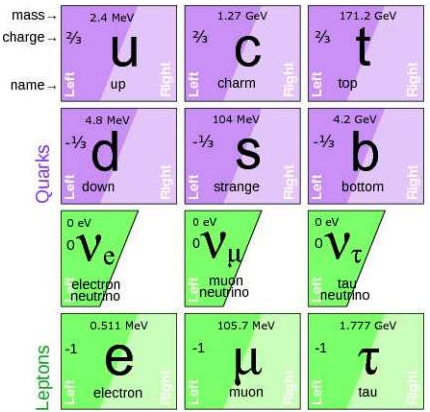
\includegraphics[width=0.90\textwidth]{./images/intro/quarks_and_leptons}
    \end{column}
    \begin{column}{0.70\textwidth}
       \begin{itemize}
         {\scriptsize
         \item 3 flavour states with LH chirality ($\nu_{eL}$, $\nu_{{\mu}L}$, $\nu_{{\tau}L}$),
               one for each charged lepton.
         \item Lepton number conserved separately in each lepton family
         \item Neutrinos have exactly zero mass
         \item Neutrinos and antineutrinos are distinct (antineutrinos are RH).
         \item They have CC and NC couplings with quarks and other leptons, given by:
         \begin{equation*}
           L^{CC} = -\frac{g}{2\sqrt{2}} j_{\mu}^{CC} W^{\mu} + h.c.
           \;\;and\;\;
           L^{NC} = -\frac{g}{2cos\theta_{w}} j_{\mu}^{NC} Z^{\mu}
         \end{equation*}
         \begin{equation*}
           where \;\;
           j_{\mu}^{CC} = 2 \sum_{e,\mu, \tau} \bar{\nu}_{{\ell}L} \gamma_{\mu} \ell_{L}
           \;\;and\;\;
           j_{\mu}^{NC} = \sum_{e,\mu, \tau} \bar{\nu}_{{\ell}L} \gamma_{\mu} \nu_{{\ell}L}
         \end{equation*}
         }
       \end{itemize}
    \end{column}
  \end{columns}

  \vspace{0.4cm}
  {\scriptsize
  The SM was constructed over the course
  of $\sim$ 20-30 yrs, since neutrinos were first proposed.\\
  \vspace{0.1cm}
  This model is now incomplete (eg. neutrinos have mass)
  but it is not clear what is the appropriate extension to the SM.
  }

\end{frame}

%
%
%

\begin{frame}[t,allowframebreaks]{Timeline of imporant events - }

\begin{itemize}
{\scriptsize

\item {\bf 1930}: The famous letter by Pauli, suggesting the existence
 of a new neutral, spin 1/2, weakly-interacting particle to salvage conservation
 of energy in $\beta$ decays.

\item {\bf 1934}: First effective theory of $\beta$ decay by Fermi
\begin{equation*}
  H_I = G_F \Big(\bar{p} \gamma^{\mu} n \Big) \Big(\bar{e} \gamma_{\mu} \nu \Big) + h.c.
\end{equation*}

\item {\bf 1934}: Calculation of neutrino-nucleus interaction cross-section
  by Bethe and Peierls.
  \begin{itemize}
  {\scriptsize
      \item Bethe: {\it "There is no practically possible way of observing the neutrino"}
      \item Pauli: {\it "I have done a terrible thing. I have postulated a particle that can not be detected."}
  }
  \end{itemize}

 \item {\bf 1946}: Pontecorvo proposed a radiochemical method for the detection of neutrino
 \begin{equation*}
   \nu + Cl^{37} \rightarrow e^{-} + Ar^{37}
 \end{equation*}

 \item {\bf 1956}: Discovery of the (anti)neutrino by Reines and Cowan
 \begin{equation*}
   \bar{\nu} + p \rightarrow e^{+} + n
 \end{equation*}

 \framebreak

 \item {\bf 1957}: Wu discovers parity violation in $\beta$ decay

 \item {\bf 1957}: Theory of massless two-component neutrino by Landau, Lee and Yang, and Salam.

 \item {\bf 1958}: Helicity of neutrino determined by Goldhaber, Grodzins and Sunyar.

 \item {\bf 1958}: Pontecorvo suggested that neutrinos have small masses,
  and the lepton number is violated in neutrino oscillations (similar to $K^0$ - $\bar{K}^0$ oscillations)

 \item {\bf 1958}: The current $\times$ current theory of weak interactions was
  proposed by Feynman and Gell-Mann, and Marshak and Sudarshan
  \begin{equation*}
    H_I = \frac{G_F}{\sqrt{2}} j^{\mu}  j_{\mu}^{\dagger}
  \end{equation*}
  where
  \begin{equation*}
    j^{\mu} = 2 \Big(\bar{p}_{L} \gamma^{\mu} n_{L} +
                     \bar{\nu}_{L} \gamma^{\mu} e_{L} +
                     \bar{\nu}_{L} \gamma^{\mu} \mu_{L} \Big)
  \end{equation*}
  is a $\mu-e$ universal CC.

  \item {\bf 1962}: Discovery of the muon neutrino by Schwartz, Lederman and Steinberger at BNL,
  in the first experiment with accelerator-made neutrinos.

  \item {\bf 1962}: Maki, Nakagawa, Sakata proposed that neutrino have masses,
  and the flavour states $\nu_e$, $\nu_{\mu}$ are connected with the fields of
  massive neutrinos $\nu_1$, $\nu_2$.
  \begin{equation}
   \nonumber
   \begin{pmatrix}
    \nu_{e L}\\ \nu_{\mu L}
   \end{pmatrix}
   =
   \begin{pmatrix}
     cos\theta & sin\theta \\
    -sin\theta & cos\theta \\
   \end{pmatrix}
   \begin{pmatrix}
    \nu_{1 L}\\ \nu_{2 L}
   \end{pmatrix}
  \end{equation}

  \framebreak

  \item {\bf 1967}: Unified Electro-weak theory by
   Glashow, Weinberg, and Salam.

  \item {\bf 1970}: Davis et al. run a pioneering experiment to detect solar
   neutrinos using the detection technique proposed by Pontecorvo.
   They observe a rate 2-3 times lower than expected.

  \item {\bf 1973}: Discovery of NC in the Gargamelle bubble
   chamber experiment at CERN.

  \item {\bf 1978}: Wolfenstein, and Mikheev and Smirnov (1986)
   estimated modifications of neutrino interactions in matter,
   and showed a resonant enhancement of mixing if the density of matter
   is slowly decreasing.

  \item {\bf 1980s}: Study of quasi-elastic and (deep)
    inelastic scattering of neutrinos on nucleons, study of form factors
    and of the quark structure of nucleons.

  \item {\bf 1987}: Observation of neutrinos from supernovae SN1987A in the
   Kamiokande, IMB and Baksan detectors.

  \item {\bf 1988}: Real time observation of (higher energy, $B^8$)
   solar neutrinos in Kamiokande, through neutrino-electron elastic scattering
   \begin{equation*}
     \nu e \rightarrow \nu e
   \end{equation*}
   The directionality of measurement demonstrated the solar origin of neutrinos.
   A lower than expected measurement of rate confirmed the solar neutrino problem.

  \item {\bf 1991}: Detection of low energy solar neutrinos via
  \begin{equation*}
    \nu_e + Ga^{71} \rightarrow e^{-} + Ge^{71}
  \end{equation*}
  by the radiochemical experiments GALLEX and SAGE shows a rate which is a factor
  of 2 lower than predicted, and largely eliminated the Standard
  Solar Model as the origin of the solar neutrino problem.

  \item {\bf 1990s}: Measurement of the $Z$ width at LEP (CERN) proves the
  existence of only 3 (light) neutrino flavours.

  \item {\bf 1998}: Measurement of atmospheric neutrino zenith angle distributions
  in Super-Kamiokande, and discovery of neutrino oscillations.

  \item {\bf 2000}: First direct observation of the $\nu_{\tau}$ by the DONuT experiment.

  \item {\bf 2002}: Separate measurements of NC and CC solar neutrino event rates
   by SNO
   \begin{equation*}
     \nu + d \rightarrow \nu + n + p
   \end{equation*}
   \begin{equation*}
     \nu_{e} + d \rightarrow e^- + p + p
   \end{equation*}
   and resolution of the solar neutrino anomaly.

  \item {\bf 2002} Confirmation of solution to the solar neutrino anomaly,
  by the KamLAND long-baseline reactor experiment.

  \item {\bf 2004} Confirmation of solution to the atmospheric neutrino problem,
  by the K2K long-baseline accelerator neutrino experiment.

  \item {\bf 2006} Confirmation of solution to the atmospheric neutrino problem,
  and precision measurement of relevant oscillation parameters
  by the MINOS long-baseline accelerator neutrino experiment.

  \item {\bf 2007} $Be^7$ solar neutrino measurement by Borexino.

  \item {\bf 2012} First measurement of $\theta_{13}$ through the study of $\bar{\nu}_e$
  disappearance in short-baseline reactor experiments Daya Bay, RENO and Double Chooz.

  \item {\bf 2014} First measurement of $\nu_{\mu} \rightarrow \nu_{e}$ by
  the T2K long-baseline accelerator neutrino experiment.

  \item {\bf 2019} First evidence for leptonic CP violation by
  the T2K long-baseline accelerator neutrino experiment.

  \item {\bf 2021} First detection of CNO neutrinos by Borexino

}
\end{itemize}

\end{frame}
